\documentclass[1p]{elsarticle_modified}
%\bibliographystyle{elsarticle-num}

%\usepackage[colorlinks]{hyperref}
%\usepackage{abbrmath_seonhwa} %\Abb, \Ascr, \Acal ,\Abf, \Afrak
\usepackage{amsfonts}
\usepackage{amssymb}
\usepackage{amsmath}
\usepackage{amsthm}
\usepackage{scalefnt}
\usepackage{amsbsy}
\usepackage{kotex}
\usepackage{caption}
\usepackage{subfig}
\usepackage{color}
\usepackage{graphicx}
\usepackage{xcolor} %% white, black, red, green, blue, cyan, magenta, yellow
\usepackage{float}
\usepackage{setspace}
\usepackage{hyperref}

\usepackage{tikz}
\usetikzlibrary{arrows}

\usepackage{multirow}
\usepackage{array} % fixed length table
\usepackage{hhline}

%%%%%%%%%%%%%%%%%%%%%
\makeatletter
\renewcommand*\env@matrix[1][\arraystretch]{%
	\edef\arraystretch{#1}%
	\hskip -\arraycolsep
	\let\@ifnextchar\new@ifnextchar
	\array{*\c@MaxMatrixCols c}}
\makeatother %https://tex.stackexchange.com/questions/14071/how-can-i-increase-the-line-spacing-in-a-matrix
%%%%%%%%%%%%%%%

\usepackage[normalem]{ulem}

\newcommand{\msout}[1]{\ifmmode\text{\sout{\ensuremath{#1}}}\else\sout{#1}\fi}
%SOURCE: \msout is \stkout macro in https://tex.stackexchange.com/questions/20609/strikeout-in-math-mode

\newcommand{\cancel}[1]{
	\ifmmode
	{\color{red}\msout{#1}}
	\else
	{\color{red}\sout{#1}}
	\fi
}

\newcommand{\add}[1]{
	{\color{blue}\uwave{#1}}
}

\newcommand{\replace}[2]{
	\ifmmode
	{\color{red}\msout{#1}}{\color{blue}\uwave{#2}}
	\else
	{\color{red}\sout{#1}}{\color{blue}\uwave{#2}}
	\fi
}

\newcommand{\Sol}{\mathcal{S}} %segment
\newcommand{\D}{D} %diagram
\newcommand{\A}{\mathcal{A}} %arc


%%%%%%%%%%%%%%%%%%%%%%%%%%%%%5 test

\def\sl{\operatorname{\textup{SL}}(2,\Cbb)}
\def\psl{\operatorname{\textup{PSL}}(2,\Cbb)}
\def\quan{\mkern 1mu \triangleright \mkern 1mu}

\theoremstyle{definition}
\newtheorem{thm}{Theorem}[section]
\newtheorem{prop}[thm]{Proposition}
\newtheorem{lem}[thm]{Lemma}
\newtheorem{ques}[thm]{Question}
\newtheorem{cor}[thm]{Corollary}
\newtheorem{defn}[thm]{Definition}
\newtheorem{exam}[thm]{Example}
\newtheorem{rmk}[thm]{Remark}
\newtheorem{alg}[thm]{Algorithm}

\newcommand{\I}{\sqrt{-1}}
\begin{document}

%\begin{frontmatter}
%
%\title{Boundary parabolic representations of knots up to 8 crossings}
%
%%% Group authors per affiliation:
%\author{Yunhi Cho} 
%\address{Department of Mathematics, University of Seoul, Seoul, Korea}
%\ead{yhcho@uos.ac.kr}
%
%
%\author{Seonhwa Kim} %\fnref{s_kim}}
%\address{Center for Geometry and Physics, Institute for Basic Science, Pohang, 37673, Korea}
%\ead{ryeona17@ibs.re.kr}
%
%\author{Hyuk Kim}
%\address{Department of Mathematical Sciences, Seoul National University, Seoul 08826, Korea}
%\ead{hyukkim@snu.ac.kr}
%
%\author{Seokbeom Yoon}
%\address{Department of Mathematical Sciences, Seoul National University, Seoul, 08826,  Korea}
%\ead{sbyoon15@snu.ac.kr}
%
%\begin{abstract}
%We find all boundary parabolic representation of knots up to 8 crossings.
%
%\end{abstract}
%\begin{keyword}
%    \MSC[2010] 57M25 
%\end{keyword}
%
%\end{frontmatter}

%\linenumbers
%\tableofcontents
%
\newcommand\colored[1]{\textcolor{white}{\rule[-0.35ex]{0.8em}{1.4ex}}\kern-0.8em\color{red} #1}%
%\newcommand\colored[1]{\textcolor{white}{ #1}\kern-2.17ex	\textcolor{white}{ #1}\kern-1.81ex	\textcolor{white}{ #1}\kern-2.15ex\color{red}#1	}

{\Large $\underline{12a_{0543}~(K12a_{0543})}$}

\setlength{\tabcolsep}{10pt}
\renewcommand{\arraystretch}{1.6}
\vspace{1cm}\begin{tabular}{m{100pt}>{\centering\arraybackslash}m{274pt}}
\multirow{5}{120pt}{
	\centering
	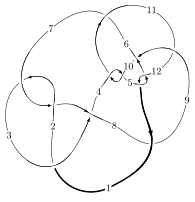
\includegraphics[width=112pt]{../../../GIT/diagram.site/Diagrams/png/1344_12a_0543.png}\\
\ \ \ A knot diagram\footnotemark}&
\allowdisplaybreaks
\textbf{Linearized knot diagam} \\
\cline{2-2}
 &
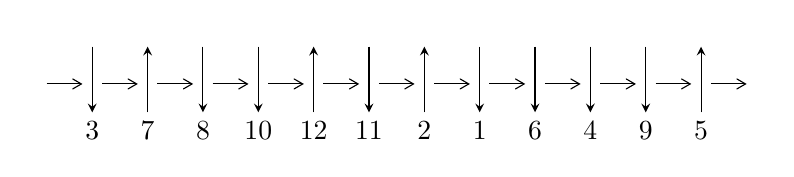
\begin{tikzpicture}[x=20pt, y=17pt]
	% nodes
	\node (C0) at (0, 0) {};
	\node (C1) at (1, 0) {};
	\node (C1U) at (1, +1) {};
	\node (C1D) at (1, -1) {3};

	\node (C2) at (2, 0) {};
	\node (C2U) at (2, +1) {};
	\node (C2D) at (2, -1) {7};

	\node (C3) at (3, 0) {};
	\node (C3U) at (3, +1) {};
	\node (C3D) at (3, -1) {8};

	\node (C4) at (4, 0) {};
	\node (C4U) at (4, +1) {};
	\node (C4D) at (4, -1) {10};

	\node (C5) at (5, 0) {};
	\node (C5U) at (5, +1) {};
	\node (C5D) at (5, -1) {12};

	\node (C6) at (6, 0) {};
	\node (C6U) at (6, +1) {};
	\node (C6D) at (6, -1) {11};

	\node (C7) at (7, 0) {};
	\node (C7U) at (7, +1) {};
	\node (C7D) at (7, -1) {2};

	\node (C8) at (8, 0) {};
	\node (C8U) at (8, +1) {};
	\node (C8D) at (8, -1) {1};

	\node (C9) at (9, 0) {};
	\node (C9U) at (9, +1) {};
	\node (C9D) at (9, -1) {6};

	\node (C10) at (10, 0) {};
	\node (C10U) at (10, +1) {};
	\node (C10D) at (10, -1) {4};

	\node (C11) at (11, 0) {};
	\node (C11U) at (11, +1) {};
	\node (C11D) at (11, -1) {9};

	\node (C12) at (12, 0) {};
	\node (C12U) at (12, +1) {};
	\node (C12D) at (12, -1) {5};
	\node (C13) at (13, 0) {};

	% arrows
	\draw[->,>={angle 60}]
	(C0) edge (C1) (C1) edge (C2) (C2) edge (C3) (C3) edge (C4) (C4) edge (C5) (C5) edge (C6) (C6) edge (C7) (C7) edge (C8) (C8) edge (C9) (C9) edge (C10) (C10) edge (C11) (C11) edge (C12) (C12) edge (C13) ;	\draw[->,>=stealth]
	(C1U) edge (C1D) (C2D) edge (C2U) (C3U) edge (C3D) (C4U) edge (C4D) (C5D) edge (C5U) (C6U) edge (C6D) (C7D) edge (C7U) (C8U) edge (C8D) (C9U) edge (C9D) (C10U) edge (C10D) (C11U) edge (C11D) (C12D) edge (C12U) ;
	\end{tikzpicture} \\
\hhline{~~} \\& 
\textbf{Solving Sequence} \\ \cline{2-2} 
 &
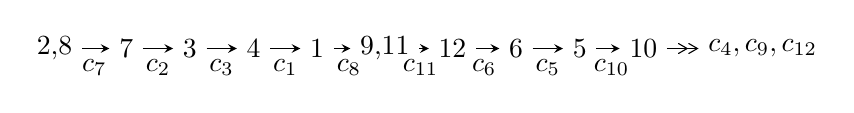
\begin{tikzpicture}[x=23pt, y=7pt]
	% node
	\node (A0) at (-1/8, 0) {2,8};
	\node (A1) at (1, 0) {7};
	\node (A2) at (2, 0) {3};
	\node (A3) at (3, 0) {4};
	\node (A4) at (4, 0) {1};
	\node (A5) at (81/16, 0) {9,11};
	\node (A6) at (49/8, 0) {12};
	\node (A7) at (57/8, 0) {6};
	\node (A8) at (65/8, 0) {5};
	\node (A9) at (73/8, 0) {10};
	\node (C1) at (1/2, -1) {$c_{7}$};
	\node (C2) at (3/2, -1) {$c_{2}$};
	\node (C3) at (5/2, -1) {$c_{3}$};
	\node (C4) at (7/2, -1) {$c_{1}$};
	\node (C5) at (9/2, -1) {$c_{8}$};
	\node (C6) at (45/8, -1) {$c_{11}$};
	\node (C7) at (53/8, -1) {$c_{6}$};
	\node (C8) at (61/8, -1) {$c_{5}$};
	\node (C9) at (69/8, -1) {$c_{10}$};
	\node (A10) at (11, 0) {$c_{4},c_{9},c_{12}$};

	% edge
	\draw[->,>=stealth]	
	(A0) edge (A1) (A1) edge (A2) (A2) edge (A3) (A3) edge (A4) (A4) edge (A5) (A5) edge (A6) (A6) edge (A7) (A7) edge (A8) (A8) edge (A9) ;
	\draw[->>,>={angle 60}]	
	(A9) edge (A10);
\end{tikzpicture} \\ 

\end{tabular} \\

\footnotetext{
The image of knot diagram is generated by the software ``\textbf{Draw programme}" developed by Andrew Bartholomew(\url{http://www.layer8.co.uk/maths/draw/index.htm\#Running-draw}), where we modified some parts for our purpose(\url{https://github.com/CATsTAILs/LinksPainter}).
}\phantom \\ \newline 
\centering \textbf{Ideals for irreducible components\footnotemark of $X_{\text{par}}$} 
 
\begin{align*}
I^u_{1}&=\langle 
1.68337\times10^{119} u^{144}+7.16684\times10^{118} u^{143}+\cdots+5.14439\times10^{118} b+6.42016\times10^{118},\\
\phantom{I^u_{1}}&\phantom{= \langle  }-1.79261\times10^{120} u^{144}-1.95501\times10^{120} u^{143}+\cdots+3.60108\times10^{119} a-8.71578\times10^{120},\\
\phantom{I^u_{1}}&\phantom{= \langle  }u^{145}+u^{144}+\cdots+10 u+7\rangle \\
I^u_{2}&=\langle 
- u^{25}- u^{24}+\cdots+b+1,\;u^{25}-2 u^{24}+\cdots+a-4,\;u^{26}+7 u^{24}+\cdots+3 u^2+1\rangle \\
\\
\end{align*}
\raggedright * 2 irreducible components of $\dim_{\mathbb{C}}=0$, with total 171 representations.\\
\footnotetext{All coefficients of polynomials are rational numbers. But the coefficients are sometimes approximated in decimal forms when there is not enough margin.}
\newpage
\renewcommand{\arraystretch}{1}
\centering \section*{I. $I^u_{1}= \langle 1.68\times10^{119} u^{144}+7.17\times10^{118} u^{143}+\cdots+5.14\times10^{118} b+6.42\times10^{118},\;-1.79\times10^{120} u^{144}-1.96\times10^{120} u^{143}+\cdots+3.60\times10^{119} a-8.72\times10^{120},\;u^{145}+u^{144}+\cdots+10 u+7 \rangle$}
\flushleft \textbf{(i) Arc colorings}\\
\begin{tabular}{m{7pt} m{180pt} m{7pt} m{180pt} }
\flushright $a_{2}=$&$\begin{pmatrix}0\\u\end{pmatrix}$ \\
\flushright $a_{8}=$&$\begin{pmatrix}1\\0\end{pmatrix}$ \\
\flushright $a_{7}=$&$\begin{pmatrix}1\\u^2\end{pmatrix}$ \\
\flushright $a_{3}=$&$\begin{pmatrix}u\\u^3+u\end{pmatrix}$ \\
\flushright $a_{4}=$&$\begin{pmatrix}- u^3\\u^3+u\end{pmatrix}$ \\
\flushright $a_{1}=$&$\begin{pmatrix}u^3\\u^5+u^3+u\end{pmatrix}$ \\
\flushright $a_{9}=$&$\begin{pmatrix}u^8+u^6+u^4+1\\u^{10}+2 u^8+3 u^6+2 u^4+u^2\end{pmatrix}$ \\
\flushright $a_{11}=$&$\begin{pmatrix}4.97800 u^{144}+5.42896 u^{143}+\cdots+56.4506 u+24.2033\\-3.27224 u^{144}-1.39314 u^{143}+\cdots-27.5746 u-1.24799\end{pmatrix}$ \\
\flushright $a_{12}=$&$\begin{pmatrix}5.49859 u^{144}+4.11098 u^{143}+\cdots+54.4352 u+13.8676\\-2.49995 u^{144}-0.367127 u^{143}+\cdots-19.0091 u+1.60456\end{pmatrix}$ \\
\flushright $a_{6}=$&$\begin{pmatrix}4.80687 u^{144}+6.35204 u^{143}+\cdots+65.5375 u+32.7772\\-2.14463 u^{144}-1.10343 u^{143}+\cdots-21.2231 u-3.92713\end{pmatrix}$ \\
\flushright $a_{5}=$&$\begin{pmatrix}2.92464 u^{144}+2.24128 u^{143}+\cdots+26.1845 u+8.46431\\0.305108 u^{144}+0.518469 u^{143}+\cdots+3.64666 u+2.19118\end{pmatrix}$ \\
\flushright $a_{10}=$&$\begin{pmatrix}5.60505 u^{144}+4.70435 u^{143}+\cdots+57.1498 u+18.1858\\-2.57136 u^{144}-0.200226 u^{143}+\cdots-17.8815 u+2.50357\end{pmatrix}$\\&\end{tabular}
\flushleft \textbf{(ii) Obstruction class $= -1$}\\~\\
\flushleft \textbf{(iii) Cusp Shapes $= 0.0931173 u^{144}+4.00522 u^{143}+\cdots+31.6281 u+25.6618$}\\~\\
\newpage\renewcommand{\arraystretch}{1}
\flushleft \textbf{(iv) u-Polynomials at the component}\newline \\
\begin{tabular}{m{50pt}|m{274pt}}
Crossings & \hspace{64pt}u-Polynomials at each crossing \\
\hline $$\begin{aligned}c_{1}\end{aligned}$$&$\begin{aligned}
&u^{145}+69 u^{144}+\cdots-362 u-49
\end{aligned}$\\
\hline $$\begin{aligned}c_{2},c_{7}\end{aligned}$$&$\begin{aligned}
&u^{145}+u^{144}+\cdots+10 u+7
\end{aligned}$\\
\hline $$\begin{aligned}c_{3}\end{aligned}$$&$\begin{aligned}
&u^{145}- u^{144}+\cdots-194332 u+20503
\end{aligned}$\\
\hline $$\begin{aligned}c_{4},c_{10}\end{aligned}$$&$\begin{aligned}
&u^{145}- u^{144}+\cdots-10727 u+2347
\end{aligned}$\\
\hline $$\begin{aligned}c_{5},c_{12}\end{aligned}$$&$\begin{aligned}
&u^{145}-2 u^{144}+\cdots-12270 u+2449
\end{aligned}$\\
\hline $$\begin{aligned}c_{6}\end{aligned}$$&$\begin{aligned}
&u^{145}+16 u^{143}+\cdots+3486694 u+149809
\end{aligned}$\\
\hline $$\begin{aligned}c_{8}\end{aligned}$$&$\begin{aligned}
&u^{145}+5 u^{144}+\cdots+35208736 u+7631659
\end{aligned}$\\
\hline $$\begin{aligned}c_{9}\end{aligned}$$&$\begin{aligned}
&u^{145}+7 u^{144}+\cdots-13 u+1
\end{aligned}$\\
\hline $$\begin{aligned}c_{11}\end{aligned}$$&$\begin{aligned}
&u^{145}-21 u^{144}+\cdots+135 u+83
\end{aligned}$\\
\hline
\end{tabular}\\~\\
\newpage\renewcommand{\arraystretch}{1}
\flushleft \textbf{(v) Riley Polynomials at the component}\newline \\
\begin{tabular}{m{50pt}|m{274pt}}
Crossings & \hspace{64pt}Riley Polynomials at each crossing \\
\hline $$\begin{aligned}c_{1}\end{aligned}$$&$\begin{aligned}
&y^{145}+21 y^{144}+\cdots-34870 y-2401
\end{aligned}$\\
\hline $$\begin{aligned}c_{2},c_{7}\end{aligned}$$&$\begin{aligned}
&y^{145}+69 y^{144}+\cdots-362 y-49
\end{aligned}$\\
\hline $$\begin{aligned}c_{3}\end{aligned}$$&$\begin{aligned}
&y^{145}-21 y^{144}+\cdots+39082161962 y-420373009
\end{aligned}$\\
\hline $$\begin{aligned}c_{4},c_{10}\end{aligned}$$&$\begin{aligned}
&y^{145}+105 y^{144}+\cdots-226926923 y-5508409
\end{aligned}$\\
\hline $$\begin{aligned}c_{5},c_{12}\end{aligned}$$&$\begin{aligned}
&y^{145}+86 y^{144}+\cdots+45603454 y-5997601
\end{aligned}$\\
\hline $$\begin{aligned}c_{6}\end{aligned}$$&$\begin{aligned}
&y^{145}+32 y^{144}+\cdots-735797446182 y-22442736481
\end{aligned}$\\
\hline $$\begin{aligned}c_{8}\end{aligned}$$&$\begin{aligned}
&y^{145}+73 y^{144}+\cdots-2911748666672046 y-58242219092281
\end{aligned}$\\
\hline $$\begin{aligned}c_{9}\end{aligned}$$&$\begin{aligned}
&y^{145}-7 y^{144}+\cdots+67 y-1
\end{aligned}$\\
\hline $$\begin{aligned}c_{11}\end{aligned}$$&$\begin{aligned}
&y^{145}-17 y^{144}+\cdots+528509 y-6889
\end{aligned}$\\
\hline
\end{tabular}\\~\\
\newpage\flushleft \textbf{(vi) Complex Volumes and Cusp Shapes}
$$\begin{array}{c|c|c}  
\text{Solutions to }I^u_{1}& \I (\text{vol} + \sqrt{-1}CS) & \text{Cusp shape}\\
 \hline 
\begin{aligned}
u &= -0.184394 + 0.997690 I \\
a &= \phantom{-}1.205560 - 0.226744 I \\
b &= -0.467031 - 0.834593 I\end{aligned}
 & -1.79715 + 1.32721 I & \phantom{-0.000000 } 0 \\ \hline\begin{aligned}
u &= -0.184394 - 0.997690 I \\
a &= \phantom{-}1.205560 + 0.226744 I \\
b &= -0.467031 + 0.834593 I\end{aligned}
 & -1.79715 - 1.32721 I & \phantom{-0.000000 } 0 \\ \hline\begin{aligned}
u &= \phantom{-}0.787390 + 0.592137 I \\
a &= -0.489679 - 0.314649 I \\
b &= -0.149224 + 0.355817 I\end{aligned}
 & \phantom{-}5.28775 - 1.33253 I & \phantom{-0.000000 } 0 \\ \hline\begin{aligned}
u &= \phantom{-}0.787390 - 0.592137 I \\
a &= -0.489679 + 0.314649 I \\
b &= -0.149224 - 0.355817 I\end{aligned}
 & \phantom{-}5.28775 + 1.33253 I & \phantom{-0.000000 } 0 \\ \hline\begin{aligned}
u &= -0.338378 + 0.957023 I \\
a &= -3.20344 + 1.10546 I \\
b &= \phantom{-}1.80339 + 1.12969 I\end{aligned}
 & -2.55022 - 4.09982 I & \phantom{-0.000000 } 0 \\ \hline\begin{aligned}
u &= -0.338378 - 0.957023 I \\
a &= -3.20344 - 1.10546 I \\
b &= \phantom{-}1.80339 - 1.12969 I\end{aligned}
 & -2.55022 + 4.09982 I & \phantom{-0.000000 } 0 \\ \hline\begin{aligned}
u &= -0.303177 + 0.976012 I \\
a &= \phantom{-}1.62753 - 0.47233 I \\
b &= -1.51906 + 0.55961 I\end{aligned}
 & \phantom{-}1.18528 - 1.07910 I & \phantom{-0.000000 } 0 \\ \hline\begin{aligned}
u &= -0.303177 - 0.976012 I \\
a &= \phantom{-}1.62753 + 0.47233 I \\
b &= -1.51906 - 0.55961 I\end{aligned}
 & \phantom{-}1.18528 + 1.07910 I & \phantom{-0.000000 } 0 \\ \hline\begin{aligned}
u &= \phantom{-}0.396214 + 0.942465 I \\
a &= -0.051002 + 0.579643 I \\
b &= -0.247222 - 0.810358 I\end{aligned}
 & -0.47939 + 1.85777 I & \phantom{-0.000000 } 0 \\ \hline\begin{aligned}
u &= \phantom{-}0.396214 - 0.942465 I \\
a &= -0.051002 - 0.579643 I \\
b &= -0.247222 + 0.810358 I\end{aligned}
 & -0.47939 - 1.85777 I & \phantom{-0.000000 } 0\\
 \hline 
 \end{array}$$\newpage$$\begin{array}{c|c|c}  
\text{Solutions to }I^u_{1}& \I (\text{vol} + \sqrt{-1}CS) & \text{Cusp shape}\\
 \hline 
\begin{aligned}
u &= -0.698321 + 0.678727 I \\
a &= -0.791006 + 0.117482 I \\
b &= -0.166137 - 0.243382 I\end{aligned}
 & \phantom{-}5.99895 - 2.02453 I & \phantom{-0.000000 } 0 \\ \hline\begin{aligned}
u &= -0.698321 - 0.678727 I \\
a &= -0.791006 - 0.117482 I \\
b &= -0.166137 + 0.243382 I\end{aligned}
 & \phantom{-}5.99895 + 2.02453 I & \phantom{-0.000000 } 0 \\ \hline\begin{aligned}
u &= -0.097852 + 1.023050 I \\
a &= \phantom{-}1.63457 - 0.39899 I \\
b &= -1.42349 - 0.63315 I\end{aligned}
 & -0.22854 + 3.12050 I & \phantom{-0.000000 } 0 \\ \hline\begin{aligned}
u &= -0.097852 - 1.023050 I \\
a &= \phantom{-}1.63457 + 0.39899 I \\
b &= -1.42349 + 0.63315 I\end{aligned}
 & -0.22854 - 3.12050 I & \phantom{-0.000000 } 0 \\ \hline\begin{aligned}
u &= \phantom{-}0.741562 + 0.623321 I \\
a &= \phantom{-}0.532405 + 0.864548 I \\
b &= \phantom{-}0.073970 - 0.745696 I\end{aligned}
 & \phantom{-}4.64179 + 11.18290 I & \phantom{-0.000000 } 0 \\ \hline\begin{aligned}
u &= \phantom{-}0.741562 - 0.623321 I \\
a &= \phantom{-}0.532405 - 0.864548 I \\
b &= \phantom{-}0.073970 + 0.745696 I\end{aligned}
 & \phantom{-}4.64179 - 11.18290 I & \phantom{-0.000000 } 0 \\ \hline\begin{aligned}
u &= \phantom{-}0.241101 + 1.005640 I \\
a &= \phantom{-}1.71508 + 1.43776 I \\
b &= -2.02337 - 0.03526 I\end{aligned}
 & \phantom{-}0.635555 + 0.338860 I & \phantom{-0.000000 } 0 \\ \hline\begin{aligned}
u &= \phantom{-}0.241101 - 1.005640 I \\
a &= \phantom{-}1.71508 - 1.43776 I \\
b &= -2.02337 + 0.03526 I\end{aligned}
 & \phantom{-}0.635555 - 0.338860 I & \phantom{-0.000000 } 0 \\ \hline\begin{aligned}
u &= \phantom{-}0.251556 + 1.022450 I \\
a &= -3.24031 + 0.24100 I \\
b &= \phantom{-}1.41535 - 1.01544 I\end{aligned}
 & -3.47507 - 2.68719 I & \phantom{-0.000000 } 0 \\ \hline\begin{aligned}
u &= \phantom{-}0.251556 - 1.022450 I \\
a &= -3.24031 - 0.24100 I \\
b &= \phantom{-}1.41535 + 1.01544 I\end{aligned}
 & -3.47507 + 2.68719 I & \phantom{-0.000000 } 0\\
 \hline 
 \end{array}$$\newpage$$\begin{array}{c|c|c}  
\text{Solutions to }I^u_{1}& \I (\text{vol} + \sqrt{-1}CS) & \text{Cusp shape}\\
 \hline 
\begin{aligned}
u &= -0.824404 + 0.433210 I \\
a &= -0.332263 - 0.322654 I \\
b &= -1.003040 + 0.868786 I\end{aligned}
 & \phantom{-}4.39588 + 2.05646 I & \phantom{-0.000000 } 0 \\ \hline\begin{aligned}
u &= -0.824404 - 0.433210 I \\
a &= -0.332263 + 0.322654 I \\
b &= -1.003040 - 0.868786 I\end{aligned}
 & \phantom{-}4.39588 - 2.05646 I & \phantom{-0.000000 } 0 \\ \hline\begin{aligned}
u &= \phantom{-}0.490005 + 0.773992 I \\
a &= \phantom{-}1.004320 + 0.687450 I \\
b &= -0.825636 - 0.474558 I\end{aligned}
 & \phantom{-}0.13695 + 2.07089 I & \phantom{-0.000000 } 0 \\ \hline\begin{aligned}
u &= \phantom{-}0.490005 - 0.773992 I \\
a &= \phantom{-}1.004320 - 0.687450 I \\
b &= -0.825636 + 0.474558 I\end{aligned}
 & \phantom{-}0.13695 - 2.07089 I & \phantom{-0.000000 } 0 \\ \hline\begin{aligned}
u &= -0.438325 + 0.992032 I \\
a &= -1.83986 - 1.03644 I \\
b &= \phantom{-}0.63602 + 2.34736 I\end{aligned}
 & -2.15013 - 6.05393 I & \phantom{-0.000000 } 0 \\ \hline\begin{aligned}
u &= -0.438325 - 0.992032 I \\
a &= -1.83986 + 1.03644 I \\
b &= \phantom{-}0.63602 - 2.34736 I\end{aligned}
 & -2.15013 + 6.05393 I & \phantom{-0.000000 } 0 \\ \hline\begin{aligned}
u &= -0.706416 + 0.581377 I \\
a &= \phantom{-}0.453554 - 0.977363 I \\
b &= \phantom{-}0.040691 + 1.056500 I\end{aligned}
 & \phantom{-}7.52331 - 5.01192 I & \phantom{-0.000000 } 0 \\ \hline\begin{aligned}
u &= -0.706416 - 0.581377 I \\
a &= \phantom{-}0.453554 + 0.977363 I \\
b &= \phantom{-}0.040691 - 1.056500 I\end{aligned}
 & \phantom{-}7.52331 + 5.01192 I & \phantom{-0.000000 } 0 \\ \hline\begin{aligned}
u &= \phantom{-}0.335392 + 1.037830 I \\
a &= \phantom{-}1.24878 + 0.94604 I \\
b &= -0.753812 + 1.170660 I\end{aligned}
 & -4.06964 + 4.22267 I & \phantom{-0.000000 } 0 \\ \hline\begin{aligned}
u &= \phantom{-}0.335392 - 1.037830 I \\
a &= \phantom{-}1.24878 - 0.94604 I \\
b &= -0.753812 - 1.170660 I\end{aligned}
 & -4.06964 - 4.22267 I & \phantom{-0.000000 } 0\\
 \hline 
 \end{array}$$\newpage$$\begin{array}{c|c|c}  
\text{Solutions to }I^u_{1}& \I (\text{vol} + \sqrt{-1}CS) & \text{Cusp shape}\\
 \hline 
\begin{aligned}
u &= \phantom{-}0.837402 + 0.346097 I \\
a &= -0.470563 + 0.071252 I \\
b &= -0.915098 - 0.992526 I\end{aligned}
 & \phantom{-}4.05564 - 4.81767 I & \phantom{-0.000000 } 0 \\ \hline\begin{aligned}
u &= \phantom{-}0.837402 - 0.346097 I \\
a &= -0.470563 - 0.071252 I \\
b &= -0.915098 + 0.992526 I\end{aligned}
 & \phantom{-}4.05564 + 4.81767 I & \phantom{-0.000000 } 0 \\ \hline\begin{aligned}
u &= -0.606369 + 0.920094 I \\
a &= -0.615571 - 0.438638 I \\
b &= -0.118732 - 0.231346 I\end{aligned}
 & \phantom{-}5.28012 - 2.99417 I & \phantom{-0.000000 } 0 \\ \hline\begin{aligned}
u &= -0.606369 - 0.920094 I \\
a &= -0.615571 + 0.438638 I \\
b &= -0.118732 + 0.231346 I\end{aligned}
 & \phantom{-}5.28012 + 2.99417 I & \phantom{-0.000000 } 0 \\ \hline\begin{aligned}
u &= -0.814299 + 0.375549 I \\
a &= \phantom{-}0.575844 + 0.635418 I \\
b &= \phantom{-}1.66703 - 1.41778 I\end{aligned}
 & \phantom{-}3.2718 + 14.1290 I & \phantom{-0.000000 } 0 \\ \hline\begin{aligned}
u &= -0.814299 - 0.375549 I \\
a &= \phantom{-}0.575844 - 0.635418 I \\
b &= \phantom{-}1.66703 + 1.41778 I\end{aligned}
 & \phantom{-}3.2718 - 14.1290 I & \phantom{-0.000000 } 0 \\ \hline\begin{aligned}
u &= -0.338107 + 0.828564 I \\
a &= \phantom{-}1.170070 + 0.396851 I \\
b &= \phantom{-}0.545917 - 1.153990 I\end{aligned}
 & -2.23687 + 1.29929 I & \phantom{-0.000000 } 0 \\ \hline\begin{aligned}
u &= -0.338107 - 0.828564 I \\
a &= \phantom{-}1.170070 - 0.396851 I \\
b &= \phantom{-}0.545917 + 1.153990 I\end{aligned}
 & -2.23687 - 1.29929 I & \phantom{-0.000000 } 0 \\ \hline\begin{aligned}
u &= \phantom{-}0.732572 + 0.502840 I \\
a &= -0.702309 - 1.007620 I \\
b &= \phantom{-}0.097958 + 0.123214 I\end{aligned}
 & \phantom{-}5.00367 + 2.20048 I & \phantom{-0.000000 } 0 \\ \hline\begin{aligned}
u &= \phantom{-}0.732572 - 0.502840 I \\
a &= -0.702309 + 1.007620 I \\
b &= \phantom{-}0.097958 - 0.123214 I\end{aligned}
 & \phantom{-}5.00367 - 2.20048 I & \phantom{-0.000000 } 0\\
 \hline 
 \end{array}$$\newpage$$\begin{array}{c|c|c}  
\text{Solutions to }I^u_{1}& \I (\text{vol} + \sqrt{-1}CS) & \text{Cusp shape}\\
 \hline 
\begin{aligned}
u &= \phantom{-}0.208756 + 1.099840 I \\
a &= \phantom{-}1.153790 + 0.284530 I \\
b &= -0.764283 + 1.064860 I\end{aligned}
 & -5.69124 - 5.08448 I & \phantom{-0.000000 } 0 \\ \hline\begin{aligned}
u &= \phantom{-}0.208756 - 1.099840 I \\
a &= \phantom{-}1.153790 - 0.284530 I \\
b &= -0.764283 - 1.064860 I\end{aligned}
 & -5.69124 + 5.08448 I & \phantom{-0.000000 } 0 \\ \hline\begin{aligned}
u &= -0.754912 + 0.442722 I \\
a &= -0.894123 - 0.814790 I \\
b &= -1.40872 + 1.09063 I\end{aligned}
 & \phantom{-}4.68617 + 4.86935 I & \phantom{-0.000000 } 0 \\ \hline\begin{aligned}
u &= -0.754912 - 0.442722 I \\
a &= -0.894123 + 0.814790 I \\
b &= -1.40872 - 1.09063 I\end{aligned}
 & \phantom{-}4.68617 - 4.86935 I & \phantom{-0.000000 } 0 \\ \hline\begin{aligned}
u &= \phantom{-}0.175228 + 1.115380 I \\
a &= -1.68414 - 1.85829 I \\
b &= \phantom{-}1.75348 + 0.18743 I\end{aligned}
 & \phantom{-}1.63161 - 5.18305 I & \phantom{-0.000000 } 0 \\ \hline\begin{aligned}
u &= \phantom{-}0.175228 - 1.115380 I \\
a &= -1.68414 + 1.85829 I \\
b &= \phantom{-}1.75348 - 0.18743 I\end{aligned}
 & \phantom{-}1.63161 + 5.18305 I & \phantom{-0.000000 } 0 \\ \hline\begin{aligned}
u &= \phantom{-}0.777707 + 0.383999 I \\
a &= \phantom{-}0.600592 - 0.714495 I \\
b &= \phantom{-}1.71002 + 1.62586 I\end{aligned}
 & \phantom{-}6.48441 - 7.60554 I & \phantom{-0.000000 } 0 \\ \hline\begin{aligned}
u &= \phantom{-}0.777707 - 0.383999 I \\
a &= \phantom{-}0.600592 + 0.714495 I \\
b &= \phantom{-}1.71002 - 1.62586 I\end{aligned}
 & \phantom{-}6.48441 + 7.60554 I & \phantom{-0.000000 } 0 \\ \hline\begin{aligned}
u &= -0.653235 + 0.563065 I \\
a &= \phantom{-}0.16315 + 1.61830 I \\
b &= \phantom{-}0.782854 - 0.672428 I\end{aligned}
 & -0.13545 - 5.31806 I & \phantom{-0.000000 } 0 \\ \hline\begin{aligned}
u &= -0.653235 - 0.563065 I \\
a &= \phantom{-}0.16315 - 1.61830 I \\
b &= \phantom{-}0.782854 + 0.672428 I\end{aligned}
 & -0.13545 + 5.31806 I & \phantom{-0.000000 } 0\\
 \hline 
 \end{array}$$\newpage$$\begin{array}{c|c|c}  
\text{Solutions to }I^u_{1}& \I (\text{vol} + \sqrt{-1}CS) & \text{Cusp shape}\\
 \hline 
\begin{aligned}
u &= -0.430800 + 1.061450 I \\
a &= -1.93162 + 0.87528 I \\
b &= \phantom{-}1.66325 + 0.81510 I\end{aligned}
 & -3.66318 - 3.44179 I & \phantom{-0.000000 } 0 \\ \hline\begin{aligned}
u &= -0.430800 - 1.061450 I \\
a &= -1.93162 - 0.87528 I \\
b &= \phantom{-}1.66325 - 0.81510 I\end{aligned}
 & -3.66318 + 3.44179 I & \phantom{-0.000000 } 0 \\ \hline\begin{aligned}
u &= -0.555844 + 1.005450 I \\
a &= -1.097740 + 0.745118 I \\
b &= \phantom{-}1.90293 + 0.12033 I\end{aligned}
 & -1.44297 + 0.59465 I & \phantom{-0.000000 } 0 \\ \hline\begin{aligned}
u &= -0.555844 - 1.005450 I \\
a &= -1.097740 - 0.745118 I \\
b &= \phantom{-}1.90293 - 0.12033 I\end{aligned}
 & -1.44297 - 0.59465 I & \phantom{-0.000000 } 0 \\ \hline\begin{aligned}
u &= -0.286561 + 1.114860 I \\
a &= -0.31602 + 1.49740 I \\
b &= \phantom{-}1.069560 - 0.389689 I\end{aligned}
 & -5.39088 + 0.00078 I & \phantom{-0.000000 } 0 \\ \hline\begin{aligned}
u &= -0.286561 - 1.114860 I \\
a &= -0.31602 - 1.49740 I \\
b &= \phantom{-}1.069560 + 0.389689 I\end{aligned}
 & -5.39088 - 0.00078 I & \phantom{-0.000000 } 0 \\ \hline\begin{aligned}
u &= \phantom{-}0.749711 + 0.373069 I \\
a &= -0.246364 + 1.321170 I \\
b &= -1.40342 - 0.51244 I\end{aligned}
 & -1.10274 - 7.51513 I & \phantom{-0.000000 } 0 \\ \hline\begin{aligned}
u &= \phantom{-}0.749711 - 0.373069 I \\
a &= -0.246364 - 1.321170 I \\
b &= -1.40342 + 0.51244 I\end{aligned}
 & -1.10274 + 7.51513 I & \phantom{-0.000000 } 0 \\ \hline\begin{aligned}
u &= \phantom{-}0.437131 + 1.077290 I \\
a &= \phantom{-}0.26927 + 1.88271 I \\
b &= -1.36581 - 1.26139 I\end{aligned}
 & -0.73593 + 1.52071 I & \phantom{-0.000000 } 0 \\ \hline\begin{aligned}
u &= \phantom{-}0.437131 - 1.077290 I \\
a &= \phantom{-}0.26927 - 1.88271 I \\
b &= -1.36581 + 1.26139 I\end{aligned}
 & -0.73593 - 1.52071 I & \phantom{-0.000000 } 0\\
 \hline 
 \end{array}$$\newpage$$\begin{array}{c|c|c}  
\text{Solutions to }I^u_{1}& \I (\text{vol} + \sqrt{-1}CS) & \text{Cusp shape}\\
 \hline 
\begin{aligned}
u &= -0.289488 + 1.127400 I \\
a &= \phantom{-}0.77596 + 1.28242 I \\
b &= \phantom{-}0.331794 - 0.970544 I\end{aligned}
 & -5.42792 + 0.17662 I & \phantom{-0.000000 } 0 \\ \hline\begin{aligned}
u &= -0.289488 - 1.127400 I \\
a &= \phantom{-}0.77596 - 1.28242 I \\
b &= \phantom{-}0.331794 + 0.970544 I\end{aligned}
 & -5.42792 - 0.17662 I & \phantom{-0.000000 } 0 \\ \hline\begin{aligned}
u &= -0.605587 + 0.994069 I \\
a &= \phantom{-}1.35475 + 0.78238 I \\
b &= -0.531018 - 0.543116 I\end{aligned}
 & \phantom{-}6.30112 - 0.02283 I & \phantom{-0.000000 } 0 \\ \hline\begin{aligned}
u &= -0.605587 - 0.994069 I \\
a &= \phantom{-}1.35475 - 0.78238 I \\
b &= -0.531018 + 0.543116 I\end{aligned}
 & \phantom{-}6.30112 + 0.02283 I & \phantom{-0.000000 } 0 \\ \hline\begin{aligned}
u &= \phantom{-}0.679698 + 0.485792 I \\
a &= \phantom{-}0.237669 - 1.035950 I \\
b &= \phantom{-}0.376722 + 0.729948 I\end{aligned}
 & \phantom{-}2.95976 + 0.92488 I & \phantom{-0.000000 } 0 \\ \hline\begin{aligned}
u &= \phantom{-}0.679698 - 0.485792 I \\
a &= \phantom{-}0.237669 + 1.035950 I \\
b &= \phantom{-}0.376722 - 0.729948 I\end{aligned}
 & \phantom{-}2.95976 - 0.92488 I & \phantom{-0.000000 } 0 \\ \hline\begin{aligned}
u &= -0.716572 + 0.425089 I \\
a &= -0.029300 - 1.060030 I \\
b &= -1.280090 + 0.563040 I\end{aligned}
 & \phantom{-}2.64102 + 3.13575 I & \phantom{-0.000000 } 0 \\ \hline\begin{aligned}
u &= -0.716572 - 0.425089 I \\
a &= -0.029300 + 1.060030 I \\
b &= -1.280090 - 0.563040 I\end{aligned}
 & \phantom{-}2.64102 - 3.13575 I & \phantom{-0.000000 } 0 \\ \hline\begin{aligned}
u &= \phantom{-}0.511208 + 0.657131 I \\
a &= \phantom{-}0.741436 + 0.404517 I \\
b &= -0.771755 - 0.186005 I\end{aligned}
 & \phantom{-}0.27239 + 1.87412 I & \phantom{-0.000000 } 0 \\ \hline\begin{aligned}
u &= \phantom{-}0.511208 - 0.657131 I \\
a &= \phantom{-}0.741436 - 0.404517 I \\
b &= -0.771755 + 0.186005 I\end{aligned}
 & \phantom{-}0.27239 - 1.87412 I & \phantom{-0.000000 } 0\\
 \hline 
 \end{array}$$\newpage$$\begin{array}{c|c|c}  
\text{Solutions to }I^u_{1}& \I (\text{vol} + \sqrt{-1}CS) & \text{Cusp shape}\\
 \hline 
\begin{aligned}
u &= \phantom{-}0.647175 + 0.971864 I \\
a &= \phantom{-}0.967998 - 0.643040 I \\
b &= -0.380814 + 0.210677 I\end{aligned}
 & \phantom{-}3.60765 - 5.91767 I & \phantom{-0.000000 } 0 \\ \hline\begin{aligned}
u &= \phantom{-}0.647175 - 0.971864 I \\
a &= \phantom{-}0.967998 + 0.643040 I \\
b &= -0.380814 - 0.210677 I\end{aligned}
 & \phantom{-}3.60765 + 5.91767 I & \phantom{-0.000000 } 0 \\ \hline\begin{aligned}
u &= -0.165538 + 1.164930 I \\
a &= -1.56610 + 1.52417 I \\
b &= \phantom{-}1.69391 - 0.15332 I\end{aligned}
 & -1.83364 + 11.47010 I & \phantom{-0.000000 } 0 \\ \hline\begin{aligned}
u &= -0.165538 - 1.164930 I \\
a &= -1.56610 - 1.52417 I \\
b &= \phantom{-}1.69391 + 0.15332 I\end{aligned}
 & -1.83364 - 11.47010 I & \phantom{-0.000000 } 0 \\ \hline\begin{aligned}
u &= \phantom{-}0.380646 + 1.117450 I \\
a &= -2.25990 - 0.29991 I \\
b &= \phantom{-}1.74240 - 0.96746 I\end{aligned}
 & -7.41429 + 5.48824 I & \phantom{-0.000000 } 0 \\ \hline\begin{aligned}
u &= \phantom{-}0.380646 - 1.117450 I \\
a &= -2.25990 + 0.29991 I \\
b &= \phantom{-}1.74240 + 0.96746 I\end{aligned}
 & -7.41429 - 5.48824 I & \phantom{-0.000000 } 0 \\ \hline\begin{aligned}
u &= \phantom{-}0.415590 + 1.106590 I \\
a &= \phantom{-}1.93053 - 0.83523 I \\
b &= -0.33602 + 1.90650 I\end{aligned}
 & -0.85504 + 5.80986 I & \phantom{-0.000000 } 0 \\ \hline\begin{aligned}
u &= \phantom{-}0.415590 - 1.106590 I \\
a &= \phantom{-}1.93053 + 0.83523 I \\
b &= -0.33602 - 1.90650 I\end{aligned}
 & -0.85504 - 5.80986 I & \phantom{-0.000000 } 0 \\ \hline\begin{aligned}
u &= \phantom{-}0.693171 + 0.424591 I \\
a &= -1.297510 + 0.408056 I \\
b &= -1.17331 - 1.38727 I\end{aligned}
 & \phantom{-}4.77635 - 1.51542 I & \phantom{-0.000000 } 0 \\ \hline\begin{aligned}
u &= \phantom{-}0.693171 - 0.424591 I \\
a &= -1.297510 - 0.408056 I \\
b &= -1.17331 + 1.38727 I\end{aligned}
 & \phantom{-}4.77635 + 1.51542 I & \phantom{-0.000000 } 0\\
 \hline 
 \end{array}$$\newpage$$\begin{array}{c|c|c}  
\text{Solutions to }I^u_{1}& \I (\text{vol} + \sqrt{-1}CS) & \text{Cusp shape}\\
 \hline 
\begin{aligned}
u &= -0.670777 + 0.453286 I \\
a &= -1.08992 + 1.00199 I \\
b &= -0.1120640 - 0.0829036 I\end{aligned}
 & \phantom{-}4.93494 + 0.50336 I & \phantom{-0.000000 } 0 \\ \hline\begin{aligned}
u &= -0.670777 - 0.453286 I \\
a &= -1.08992 - 1.00199 I \\
b &= -0.1120640 + 0.0829036 I\end{aligned}
 & \phantom{-}4.93494 - 0.50336 I & \phantom{-0.000000 } 0 \\ \hline\begin{aligned}
u &= -0.658657 + 0.469439 I \\
a &= \phantom{-}0.155719 + 0.370369 I \\
b &= \phantom{-}2.14970 - 0.34783 I\end{aligned}
 & \phantom{-}0.96555 - 2.70815 I & \phantom{-0.000000 } 0 \\ \hline\begin{aligned}
u &= -0.658657 - 0.469439 I \\
a &= \phantom{-}0.155719 - 0.370369 I \\
b &= \phantom{-}2.14970 + 0.34783 I\end{aligned}
 & \phantom{-}0.96555 + 2.70815 I & \phantom{-0.000000 } 0 \\ \hline\begin{aligned}
u &= \phantom{-}0.696152 + 0.409095 I \\
a &= \phantom{-}0.023956 + 0.141789 I \\
b &= \phantom{-}1.85277 - 0.60815 I\end{aligned}
 & \phantom{-}0.66094 - 4.68741 I & \phantom{-0.000000 } 0 \\ \hline\begin{aligned}
u &= \phantom{-}0.696152 - 0.409095 I \\
a &= \phantom{-}0.023956 - 0.141789 I \\
b &= \phantom{-}1.85277 + 0.60815 I\end{aligned}
 & \phantom{-}0.66094 + 4.68741 I & \phantom{-0.000000 } 0 \\ \hline\begin{aligned}
u &= \phantom{-}0.569625 + 1.050860 I \\
a &= -1.096000 - 0.096015 I \\
b &= \phantom{-}1.187160 - 0.449559 I\end{aligned}
 & \phantom{-}1.29070 + 3.91656 I & \phantom{-0.000000 } 0 \\ \hline\begin{aligned}
u &= \phantom{-}0.569625 - 1.050860 I \\
a &= -1.096000 + 0.096015 I \\
b &= \phantom{-}1.187160 + 0.449559 I\end{aligned}
 & \phantom{-}1.29070 - 3.91656 I & \phantom{-0.000000 } 0 \\ \hline\begin{aligned}
u &= \phantom{-}0.530351 + 1.072130 I \\
a &= \phantom{-}2.15831 + 1.00377 I \\
b &= -2.27909 + 0.16677 I\end{aligned}
 & -2.70997 + 2.55761 I & \phantom{-0.000000 } 0 \\ \hline\begin{aligned}
u &= \phantom{-}0.530351 - 1.072130 I \\
a &= \phantom{-}2.15831 - 1.00377 I \\
b &= -2.27909 - 0.16677 I\end{aligned}
 & -2.70997 - 2.55761 I & \phantom{-0.000000 } 0\\
 \hline 
 \end{array}$$\newpage$$\begin{array}{c|c|c}  
\text{Solutions to }I^u_{1}& \I (\text{vol} + \sqrt{-1}CS) & \text{Cusp shape}\\
 \hline 
\begin{aligned}
u &= -0.560721 + 1.056780 I \\
a &= -1.99582 + 2.46246 I \\
b &= \phantom{-}2.59318 + 0.22613 I\end{aligned}
 & -0.76533 - 2.05228 I & \phantom{-0.000000 } 0 \\ \hline\begin{aligned}
u &= -0.560721 - 1.056780 I \\
a &= -1.99582 - 2.46246 I \\
b &= \phantom{-}2.59318 - 0.22613 I\end{aligned}
 & -0.76533 + 2.05228 I & \phantom{-0.000000 } 0 \\ \hline\begin{aligned}
u &= -0.072536 + 1.198540 I \\
a &= \phantom{-}0.843928 - 0.674907 I \\
b &= -0.859816 + 0.260701 I\end{aligned}
 & -1.223970 - 0.253168 I & \phantom{-0.000000 } 0 \\ \hline\begin{aligned}
u &= -0.072536 - 1.198540 I \\
a &= \phantom{-}0.843928 + 0.674907 I \\
b &= -0.859816 - 0.260701 I\end{aligned}
 & -1.223970 + 0.253168 I & \phantom{-0.000000 } 0 \\ \hline\begin{aligned}
u &= \phantom{-}0.665080 + 1.003710 I \\
a &= -0.527424 + 0.347058 I \\
b &= -0.0028840 + 0.0612795 I\end{aligned}
 & \phantom{-}4.06228 + 6.77781 I & \phantom{-0.000000 } 0 \\ \hline\begin{aligned}
u &= \phantom{-}0.665080 - 1.003710 I \\
a &= -0.527424 - 0.347058 I \\
b &= -0.0028840 - 0.0612795 I\end{aligned}
 & \phantom{-}4.06228 - 6.77781 I & \phantom{-0.000000 } 0 \\ \hline\begin{aligned}
u &= -0.564275 + 1.065810 I \\
a &= -0.106865 - 0.291564 I \\
b &= \phantom{-}0.186769 - 0.738135 I\end{aligned}
 & \phantom{-}3.13220 - 5.30727 I & \phantom{-0.000000 } 0 \\ \hline\begin{aligned}
u &= -0.564275 - 1.065810 I \\
a &= -0.106865 + 0.291564 I \\
b &= \phantom{-}0.186769 + 0.738135 I\end{aligned}
 & \phantom{-}3.13220 + 5.30727 I & \phantom{-0.000000 } 0 \\ \hline\begin{aligned}
u &= \phantom{-}0.602451 + 1.051580 I \\
a &= -0.297227 + 0.108546 I \\
b &= \phantom{-}0.495009 + 0.529668 I\end{aligned}
 & \phantom{-}3.37666 + 2.89310 I & \phantom{-0.000000 } 0 \\ \hline\begin{aligned}
u &= \phantom{-}0.602451 - 1.051580 I \\
a &= -0.297227 - 0.108546 I \\
b &= \phantom{-}0.495009 - 0.529668 I\end{aligned}
 & \phantom{-}3.37666 - 2.89310 I & \phantom{-0.000000 } 0\\
 \hline 
 \end{array}$$\newpage$$\begin{array}{c|c|c}  
\text{Solutions to }I^u_{1}& \I (\text{vol} + \sqrt{-1}CS) & \text{Cusp shape}\\
 \hline 
\begin{aligned}
u &= -0.786073 + 0.018603 I \\
a &= -0.134255 + 0.444436 I \\
b &= -0.648623 + 1.033690 I\end{aligned}
 & -1.84816 + 6.47339 I & -4.00000 - 7.35991 I \\ \hline\begin{aligned}
u &= -0.786073 - 0.018603 I \\
a &= -0.134255 - 0.444436 I \\
b &= -0.648623 - 1.033690 I\end{aligned}
 & -1.84816 - 6.47339 I & -4.00000 + 7.35991 I \\ \hline\begin{aligned}
u &= \phantom{-}0.470849 + 1.123390 I \\
a &= -1.16024 - 1.31564 I \\
b &= \phantom{-}1.53168 - 0.31962 I\end{aligned}
 & -6.80529 + 2.18799 I & \phantom{-0.000000 } 0 \\ \hline\begin{aligned}
u &= \phantom{-}0.470849 - 1.123390 I \\
a &= -1.16024 + 1.31564 I \\
b &= \phantom{-}1.53168 + 0.31962 I\end{aligned}
 & -6.80529 - 2.18799 I & \phantom{-0.000000 } 0 \\ \hline\begin{aligned}
u &= \phantom{-}0.569536 + 1.079360 I \\
a &= \phantom{-}2.37858 + 0.41773 I \\
b &= -1.89509 + 1.91867 I\end{aligned}
 & \phantom{-}2.85729 + 6.39098 I & \phantom{-0.000000 } 0 \\ \hline\begin{aligned}
u &= \phantom{-}0.569536 - 1.079360 I \\
a &= \phantom{-}2.37858 - 0.41773 I \\
b &= -1.89509 - 1.91867 I\end{aligned}
 & \phantom{-}2.85729 - 6.39098 I & \phantom{-0.000000 } 0 \\ \hline\begin{aligned}
u &= -0.720675 + 0.285629 I \\
a &= \phantom{-}0.532398 + 0.003468 I \\
b &= -0.300937 - 1.176800 I\end{aligned}
 & -1.27972 + 3.13142 I & -4.00000 + 1.52364 I \\ \hline\begin{aligned}
u &= -0.720675 - 0.285629 I \\
a &= \phantom{-}0.532398 - 0.003468 I \\
b &= -0.300937 + 1.176800 I\end{aligned}
 & -1.27972 - 3.13142 I & -4.00000 - 1.52364 I \\ \hline\begin{aligned}
u &= \phantom{-}0.566972 + 1.085860 I \\
a &= -0.72019 - 2.70277 I \\
b &= \phantom{-}1.95871 + 0.64288 I\end{aligned}
 & -1.31995 + 9.55890 I & \phantom{-0.000000 } 0 \\ \hline\begin{aligned}
u &= \phantom{-}0.566972 - 1.085860 I \\
a &= -0.72019 + 2.70277 I \\
b &= \phantom{-}1.95871 - 0.64288 I\end{aligned}
 & -1.31995 - 9.55890 I & \phantom{-0.000000 } 0\\
 \hline 
 \end{array}$$\newpage$$\begin{array}{c|c|c}  
\text{Solutions to }I^u_{1}& \I (\text{vol} + \sqrt{-1}CS) & \text{Cusp shape}\\
 \hline 
\begin{aligned}
u &= -0.577640 + 1.082700 I \\
a &= \phantom{-}1.71775 - 1.10252 I \\
b &= -2.09488 - 0.26553 I\end{aligned}
 & \phantom{-}0.70880 - 8.09519 I & \phantom{-0.000000 } 0 \\ \hline\begin{aligned}
u &= -0.577640 - 1.082700 I \\
a &= \phantom{-}1.71775 + 1.10252 I \\
b &= -2.09488 + 0.26553 I\end{aligned}
 & \phantom{-}0.70880 + 8.09519 I & \phantom{-0.000000 } 0 \\ \hline\begin{aligned}
u &= -0.545457 + 1.112530 I \\
a &= -2.17887 - 0.42343 I \\
b &= \phantom{-}1.35181 + 1.72217 I\end{aligned}
 & -3.64516 - 7.56566 I & \phantom{-0.000000 } 0 \\ \hline\begin{aligned}
u &= -0.545457 - 1.112530 I \\
a &= -2.17887 + 0.42343 I \\
b &= \phantom{-}1.35181 - 1.72217 I\end{aligned}
 & -3.64516 + 7.56566 I & \phantom{-0.000000 } 0 \\ \hline\begin{aligned}
u &= -0.597023 + 1.086030 I \\
a &= \phantom{-}2.15158 - 0.82628 I \\
b &= -2.26804 - 1.36181 I\end{aligned}
 & \phantom{-}2.78055 - 9.99731 I & \phantom{-0.000000 } 0 \\ \hline\begin{aligned}
u &= -0.597023 - 1.086030 I \\
a &= \phantom{-}2.15158 + 0.82628 I \\
b &= -2.26804 + 1.36181 I\end{aligned}
 & \phantom{-}2.78055 + 9.99731 I & \phantom{-0.000000 } 0 \\ \hline\begin{aligned}
u &= \phantom{-}0.193774 + 1.229020 I \\
a &= \phantom{-}0.752680 + 0.881514 I \\
b &= -1.067280 - 0.404511 I\end{aligned}
 & -1.11956 - 1.75849 I & \phantom{-0.000000 } 0 \\ \hline\begin{aligned}
u &= \phantom{-}0.193774 - 1.229020 I \\
a &= \phantom{-}0.752680 - 0.881514 I \\
b &= -1.067280 + 0.404511 I\end{aligned}
 & -1.11956 + 1.75849 I & \phantom{-0.000000 } 0 \\ \hline\begin{aligned}
u &= -0.687980 + 0.303581 I \\
a &= \phantom{-}0.814867 + 0.487323 I \\
b &= \phantom{-}0.62146 - 1.37978 I\end{aligned}
 & -1.33531 + 2.81897 I & -6.12249 - 2.40079 I \\ \hline\begin{aligned}
u &= -0.687980 - 0.303581 I \\
a &= \phantom{-}0.814867 - 0.487323 I \\
b &= \phantom{-}0.62146 + 1.37978 I\end{aligned}
 & -1.33531 - 2.81897 I & -6.12249 + 2.40079 I\\
 \hline 
 \end{array}$$\newpage$$\begin{array}{c|c|c}  
\text{Solutions to }I^u_{1}& \I (\text{vol} + \sqrt{-1}CS) & \text{Cusp shape}\\
 \hline 
\begin{aligned}
u &= -0.543472 + 1.126620 I \\
a &= -1.00340 - 1.43746 I \\
b &= -0.18736 + 1.58829 I\end{aligned}
 & -3.71059 - 7.93725 I & \phantom{-0.000000 } 0 \\ \hline\begin{aligned}
u &= -0.543472 - 1.126620 I \\
a &= -1.00340 + 1.43746 I \\
b &= -0.18736 - 1.58829 I\end{aligned}
 & -3.71059 + 7.93725 I & \phantom{-0.000000 } 0 \\ \hline\begin{aligned}
u &= \phantom{-}0.576970 + 1.110150 I \\
a &= \phantom{-}1.77781 + 1.07541 I \\
b &= -2.38634 + 0.30525 I\end{aligned}
 & -3.26812 + 12.54560 I & \phantom{-0.000000 } 0 \\ \hline\begin{aligned}
u &= \phantom{-}0.576970 - 1.110150 I \\
a &= \phantom{-}1.77781 - 1.07541 I \\
b &= -2.38634 - 0.30525 I\end{aligned}
 & -3.26812 - 12.54560 I & \phantom{-0.000000 } 0 \\ \hline\begin{aligned}
u &= -0.439519 + 1.177620 I \\
a &= \phantom{-}1.60063 + 0.53610 I \\
b &= -0.58033 - 1.55254 I\end{aligned}
 & -5.28717 - 10.80720 I & \phantom{-0.000000 } 0 \\ \hline\begin{aligned}
u &= -0.439519 - 1.177620 I \\
a &= \phantom{-}1.60063 - 0.53610 I \\
b &= -0.58033 + 1.55254 I\end{aligned}
 & -5.28717 + 10.80720 I & \phantom{-0.000000 } 0 \\ \hline\begin{aligned}
u &= \phantom{-}0.588713 + 1.114710 I \\
a &= -3.04785 - 0.61947 I \\
b &= \phantom{-}2.45496 - 1.83511 I\end{aligned}
 & \phantom{-}4.32194 + 12.75140 I & \phantom{-0.000000 } 0 \\ \hline\begin{aligned}
u &= \phantom{-}0.588713 - 1.114710 I \\
a &= -3.04785 + 0.61947 I \\
b &= \phantom{-}2.45496 + 1.83511 I\end{aligned}
 & \phantom{-}4.32194 - 12.75140 I & \phantom{-0.000000 } 0 \\ \hline\begin{aligned}
u &= -0.409051 + 1.195690 I \\
a &= \phantom{-}0.245838 - 1.307360 I \\
b &= -1.061410 + 0.867196 I\end{aligned}
 & -5.50406 + 2.24792 I & \phantom{-0.000000 } 0 \\ \hline\begin{aligned}
u &= -0.409051 - 1.195690 I \\
a &= \phantom{-}0.245838 + 1.307360 I \\
b &= -1.061410 - 0.867196 I\end{aligned}
 & -5.50406 - 2.24792 I & \phantom{-0.000000 } 0\\
 \hline 
 \end{array}$$\newpage$$\begin{array}{c|c|c}  
\text{Solutions to }I^u_{1}& \I (\text{vol} + \sqrt{-1}CS) & \text{Cusp shape}\\
 \hline 
\begin{aligned}
u &= -0.621234 + 1.107540 I \\
a &= \phantom{-}1.59139 - 0.60187 I \\
b &= -1.45625 - 0.90520 I\end{aligned}
 & \phantom{-}2.37877 - 7.44465 I & \phantom{-0.000000 } 0 \\ \hline\begin{aligned}
u &= -0.621234 - 1.107540 I \\
a &= \phantom{-}1.59139 + 0.60187 I \\
b &= -1.45625 + 0.90520 I\end{aligned}
 & \phantom{-}2.37877 + 7.44465 I & \phantom{-0.000000 } 0 \\ \hline\begin{aligned}
u &= -0.598688 + 1.129240 I \\
a &= -2.70720 + 0.66114 I \\
b &= \phantom{-}2.33879 + 1.64430 I\end{aligned}
 & \phantom{-}1.0265 - 19.4036 I & \phantom{-0.000000 } 0 \\ \hline\begin{aligned}
u &= -0.598688 - 1.129240 I \\
a &= -2.70720 - 0.66114 I \\
b &= \phantom{-}2.33879 - 1.64430 I\end{aligned}
 & \phantom{-}1.0265 + 19.4036 I & \phantom{-0.000000 } 0 \\ \hline\begin{aligned}
u &= \phantom{-}0.599077 + 1.144460 I \\
a &= \phantom{-}1.64688 + 0.30692 I \\
b &= -1.26606 + 1.23218 I\end{aligned}
 & \phantom{-}1.67753 + 10.14400 I & \phantom{-0.000000 } 0 \\ \hline\begin{aligned}
u &= \phantom{-}0.599077 - 1.144460 I \\
a &= \phantom{-}1.64688 - 0.30692 I \\
b &= -1.26606 - 1.23218 I\end{aligned}
 & \phantom{-}1.67753 - 10.14400 I & \phantom{-0.000000 } 0 \\ \hline\begin{aligned}
u &= \phantom{-}0.568890 + 0.385452 I \\
a &= \phantom{-}0.54032 + 1.67742 I \\
b &= -1.251310 - 0.652831 I\end{aligned}
 & -0.75101 + 1.90370 I & -4.80872 - 0.09845 I \\ \hline\begin{aligned}
u &= \phantom{-}0.568890 - 0.385452 I \\
a &= \phantom{-}0.54032 - 1.67742 I \\
b &= -1.251310 + 0.652831 I\end{aligned}
 & -0.75101 - 1.90370 I & -4.80872 + 0.09845 I \\ \hline\begin{aligned}
u &= \phantom{-}0.642939 + 0.120216 I \\
a &= \phantom{-}0.566798 + 0.181916 I \\
b &= \phantom{-}1.162810 - 0.332187 I\end{aligned}
 & -4.02495 + 2.01618 I & -7.90744 - 1.24994 I \\ \hline\begin{aligned}
u &= \phantom{-}0.642939 - 0.120216 I \\
a &= \phantom{-}0.566798 - 0.181916 I \\
b &= \phantom{-}1.162810 + 0.332187 I\end{aligned}
 & -4.02495 - 2.01618 I & -7.90744 + 1.24994 I\\
 \hline 
 \end{array}$$\newpage$$\begin{array}{c|c|c}  
\text{Solutions to }I^u_{1}& \I (\text{vol} + \sqrt{-1}CS) & \text{Cusp shape}\\
 \hline 
\begin{aligned}
u &= \phantom{-}0.593300 + 0.022047 I \\
a &= -0.101191 - 1.046710 I \\
b &= -0.607461 - 1.118300 I\end{aligned}
 & \phantom{-}2.10728 - 2.09321 I & \phantom{-}0.33268 + 3.77036 I \\ \hline\begin{aligned}
u &= \phantom{-}0.593300 - 0.022047 I \\
a &= -0.101191 + 1.046710 I \\
b &= -0.607461 + 1.118300 I\end{aligned}
 & \phantom{-}2.10728 + 2.09321 I & \phantom{-}0.33268 - 3.77036 I \\ \hline\begin{aligned}
u &= -0.331001 + 0.427874 I \\
a &= \phantom{-}2.29469 + 0.54871 I \\
b &= -0.286337 - 1.291110 I\end{aligned}
 & -0.66545 + 2.55610 I & -0.94084 - 2.48924 I \\ \hline\begin{aligned}
u &= -0.331001 - 0.427874 I \\
a &= \phantom{-}2.29469 - 0.54871 I \\
b &= -0.286337 + 1.291110 I\end{aligned}
 & -0.66545 - 2.55610 I & -0.94084 + 2.48924 I \\ \hline\begin{aligned}
u &= -0.461079\phantom{ +0.000000I} \\
a &= \phantom{-}0.707907\phantom{ +0.000000I} \\
b &= \phantom{-}0.893156\phantom{ +0.000000I}\end{aligned}
 & -1.10691\phantom{ +0.000000I} & -8.89040\phantom{ +0.000000I}\\
 \hline 
 \end{array}$$\newpage\newpage\renewcommand{\arraystretch}{1}
\centering \section*{II. $I^u_{2}= \langle - u^{25}- u^{24}+\cdots+b+1,\;u^{25}-2 u^{24}+\cdots+a-4,\;u^{26}+7 u^{24}+\cdots+3 u^2+1 \rangle$}
\flushleft \textbf{(i) Arc colorings}\\
\begin{tabular}{m{7pt} m{180pt} m{7pt} m{180pt} }
\flushright $a_{2}=$&$\begin{pmatrix}0\\u\end{pmatrix}$ \\
\flushright $a_{8}=$&$\begin{pmatrix}1\\0\end{pmatrix}$ \\
\flushright $a_{7}=$&$\begin{pmatrix}1\\u^2\end{pmatrix}$ \\
\flushright $a_{3}=$&$\begin{pmatrix}u\\u^3+u\end{pmatrix}$ \\
\flushright $a_{4}=$&$\begin{pmatrix}- u^3\\u^3+u\end{pmatrix}$ \\
\flushright $a_{1}=$&$\begin{pmatrix}u^3\\u^5+u^3+u\end{pmatrix}$ \\
\flushright $a_{9}=$&$\begin{pmatrix}u^8+u^6+u^4+1\\u^{10}+2 u^8+3 u^6+2 u^4+u^2\end{pmatrix}$ \\
\flushright $a_{11}=$&$\begin{pmatrix}- u^{25}+2 u^{24}+\cdots+6 u^2+4\\u^{25}+u^{24}+\cdots+u-1\end{pmatrix}$ \\
\flushright $a_{12}=$&$\begin{pmatrix}- u^{25}+u^{24}+\cdots+4 u^2+3\\u^{25}+u^{24}+\cdots+u-1\end{pmatrix}$ \\
\flushright $a_{6}=$&$\begin{pmatrix}u^{25}+u^{24}+\cdots+2 u+1\\u^{25}- u^{24}+\cdots-2 u^2-2\end{pmatrix}$ \\
\flushright $a_{5}=$&$\begin{pmatrix}-2 u^{23}+u^{22}+\cdots-6 u^3-4 u\\- u^{25}-6 u^{23}+\cdots+u^4+u\end{pmatrix}$ \\
\flushright $a_{10}=$&$\begin{pmatrix}- u^{25}+u^{24}+\cdots+3 u^2+3\\u^{25}+u^{24}+\cdots- u^4+u\end{pmatrix}$\\&\end{tabular}
\flushleft \textbf{(ii) Obstruction class $= 1$}\\~\\
\flushleft \textbf{(iii) Cusp Shapes $= 13 u^{25}+86 u^{23}-2 u^{22}+287 u^{21}-12 u^{20}+605 u^{19}-37 u^{18}+877 u^{17}-71 u^{16}+918 u^{15}-80 u^{14}+740 u^{13}-40 u^{12}+515 u^{11}+30 u^{10}+337 u^9+66 u^8+177 u^7+53 u^6+58 u^5+17 u^4+16 u^3-5 u^2+10 u-9$}\\~\\
\newpage\renewcommand{\arraystretch}{1}
\flushleft \textbf{(iv) u-Polynomials at the component}\newline \\
\begin{tabular}{m{50pt}|m{274pt}}
Crossings & \hspace{64pt}u-Polynomials at each crossing \\
\hline $$\begin{aligned}c_{1}\end{aligned}$$&$\begin{aligned}
&u^{26}-14 u^{25}+\cdots-6 u+1
\end{aligned}$\\
\hline $$\begin{aligned}c_{2}\end{aligned}$$&$\begin{aligned}
&u^{26}+7 u^{24}+\cdots+3 u^2+1
\end{aligned}$\\
\hline $$\begin{aligned}c_{3}\end{aligned}$$&$\begin{aligned}
&u^{26}-2 u^{24}+\cdots-2 u+1
\end{aligned}$\\
\hline $$\begin{aligned}c_{4}\end{aligned}$$&$\begin{aligned}
&u^{26}+13 u^{24}+\cdots- u+1
\end{aligned}$\\
\hline $$\begin{aligned}c_{5}\end{aligned}$$&$\begin{aligned}
&u^{26}+u^{25}+\cdots+13 u^2+1
\end{aligned}$\\
\hline $$\begin{aligned}c_{6}\end{aligned}$$&$\begin{aligned}
&u^{26}+u^{25}+\cdots-2 u+1
\end{aligned}$\\
\hline $$\begin{aligned}c_{7}\end{aligned}$$&$\begin{aligned}
&u^{26}+7 u^{24}+\cdots+3 u^2+1
\end{aligned}$\\
\hline $$\begin{aligned}c_{8}\end{aligned}$$&$\begin{aligned}
&u^{26}+7 u^{24}+\cdots+3 u^2+1
\end{aligned}$\\
\hline $$\begin{aligned}c_{9}\end{aligned}$$&$\begin{aligned}
&u^{26}+2 u^{25}+\cdots- u+1
\end{aligned}$\\
\hline $$\begin{aligned}c_{10}\end{aligned}$$&$\begin{aligned}
&u^{26}+13 u^{24}+\cdots+u+1
\end{aligned}$\\
\hline $$\begin{aligned}c_{11}\end{aligned}$$&$\begin{aligned}
&u^{26}-4 u^{24}+\cdots+7 u+1
\end{aligned}$\\
\hline $$\begin{aligned}c_{12}\end{aligned}$$&$\begin{aligned}
&u^{26}- u^{25}+\cdots+13 u^2+1
\end{aligned}$\\
\hline
\end{tabular}\\~\\
\newpage\renewcommand{\arraystretch}{1}
\flushleft \textbf{(v) Riley Polynomials at the component}\newline \\
\begin{tabular}{m{50pt}|m{274pt}}
Crossings & \hspace{64pt}Riley Polynomials at each crossing \\
\hline $$\begin{aligned}c_{1}\end{aligned}$$&$\begin{aligned}
&y^{26}+2 y^{25}+\cdots+10 y+1
\end{aligned}$\\
\hline $$\begin{aligned}c_{2},c_{7}\end{aligned}$$&$\begin{aligned}
&y^{26}+14 y^{25}+\cdots+6 y+1
\end{aligned}$\\
\hline $$\begin{aligned}c_{3}\end{aligned}$$&$\begin{aligned}
&y^{26}-4 y^{25}+\cdots+6 y+1
\end{aligned}$\\
\hline $$\begin{aligned}c_{4},c_{10}\end{aligned}$$&$\begin{aligned}
&y^{26}+26 y^{25}+\cdots+19 y+1
\end{aligned}$\\
\hline $$\begin{aligned}c_{5},c_{12}\end{aligned}$$&$\begin{aligned}
&y^{26}+19 y^{25}+\cdots+26 y+1
\end{aligned}$\\
\hline $$\begin{aligned}c_{6}\end{aligned}$$&$\begin{aligned}
&y^{26}-7 y^{25}+\cdots-2 y+1
\end{aligned}$\\
\hline $$\begin{aligned}c_{8}\end{aligned}$$&$\begin{aligned}
&y^{26}+14 y^{25}+\cdots+6 y+1
\end{aligned}$\\
\hline $$\begin{aligned}c_{9}\end{aligned}$$&$\begin{aligned}
&y^{26}-2 y^{25}+\cdots-7 y+1
\end{aligned}$\\
\hline $$\begin{aligned}c_{11}\end{aligned}$$&$\begin{aligned}
&y^{26}-8 y^{25}+\cdots-5 y+1
\end{aligned}$\\
\hline
\end{tabular}\\~\\
\newpage\flushleft \textbf{(vi) Complex Volumes and Cusp Shapes}
$$\begin{array}{c|c|c}  
\text{Solutions to }I^u_{2}& \I (\text{vol} + \sqrt{-1}CS) & \text{Cusp shape}\\
 \hline 
\begin{aligned}
u &= -0.359440 + 0.910887 I \\
a &= \phantom{-}1.77754 - 1.04325 I \\
b &= -1.84702 + 0.56243 I\end{aligned}
 & \phantom{-}1.81449 - 1.47433 I & \phantom{-}2.93751 + 5.13499 I \\ \hline\begin{aligned}
u &= -0.359440 - 0.910887 I \\
a &= \phantom{-}1.77754 + 1.04325 I \\
b &= -1.84702 - 0.56243 I\end{aligned}
 & \phantom{-}1.81449 + 1.47433 I & \phantom{-}2.93751 - 5.13499 I \\ \hline\begin{aligned}
u &= \phantom{-}0.402070 + 1.012970 I \\
a &= -2.58496 - 0.45894 I \\
b &= \phantom{-}1.39908 - 1.96159 I\end{aligned}
 & -3.09604 + 5.11284 I & -9.28335 - 9.03985 I \\ \hline\begin{aligned}
u &= \phantom{-}0.402070 - 1.012970 I \\
a &= -2.58496 + 0.45894 I \\
b &= \phantom{-}1.39908 + 1.96159 I\end{aligned}
 & -3.09604 - 5.11284 I & -9.28335 + 9.03985 I \\ \hline\begin{aligned}
u &= \phantom{-}0.789971 + 0.415474 I \\
a &= -0.627696 + 0.302463 I \\
b &= -1.087560 - 0.836873 I\end{aligned}
 & \phantom{-}4.28502 - 3.71076 I & -0.33164 + 1.61195 I \\ \hline\begin{aligned}
u &= \phantom{-}0.789971 - 0.415474 I \\
a &= -0.627696 - 0.302463 I \\
b &= -1.087560 + 0.836873 I\end{aligned}
 & \phantom{-}4.28502 + 3.71076 I & -0.33164 - 1.61195 I \\ \hline\begin{aligned}
u &= -0.699594 + 0.550884 I \\
a &= -0.956695 + 0.481873 I \\
b &= -0.200902 + 0.037955 I\end{aligned}
 & \phantom{-}5.12297 - 1.01125 I & \phantom{-}0.66466 + 1.43973 I \\ \hline\begin{aligned}
u &= -0.699594 - 0.550884 I \\
a &= -0.956695 - 0.481873 I \\
b &= -0.200902 - 0.037955 I\end{aligned}
 & \phantom{-}5.12297 + 1.01125 I & \phantom{-}0.66466 - 1.43973 I \\ \hline\begin{aligned}
u &= \phantom{-}0.510275 + 1.047840 I \\
a &= -1.71620 - 2.34544 I \\
b &= \phantom{-}2.66024 + 0.58919 I\end{aligned}
 & -2.28523 + 1.24764 I & -9.11702 + 0.85683 I \\ \hline\begin{aligned}
u &= \phantom{-}0.510275 - 1.047840 I \\
a &= -1.71620 + 2.34544 I \\
b &= \phantom{-}2.66024 - 0.58919 I\end{aligned}
 & -2.28523 - 1.24764 I & -9.11702 - 0.85683 I\\
 \hline 
 \end{array}$$\newpage$$\begin{array}{c|c|c}  
\text{Solutions to }I^u_{2}& \I (\text{vol} + \sqrt{-1}CS) & \text{Cusp shape}\\
 \hline 
\begin{aligned}
u &= -0.339378 + 1.125810 I \\
a &= -0.826794 - 0.820362 I \\
b &= -0.365525 + 0.879813 I\end{aligned}
 & -5.01673 + 0.90484 I & -7.57121 - 2.48547 I \\ \hline\begin{aligned}
u &= -0.339378 - 1.125810 I \\
a &= -0.826794 + 0.820362 I \\
b &= -0.365525 - 0.879813 I\end{aligned}
 & -5.01673 - 0.90484 I & -7.57121 + 2.48547 I \\ \hline\begin{aligned}
u &= -0.585961 + 1.027330 I \\
a &= \phantom{-}0.071777 - 0.307147 I \\
b &= -0.069106 - 0.778948 I\end{aligned}
 & \phantom{-}3.69821 - 3.93735 I & -0.59875 + 3.86614 I \\ \hline\begin{aligned}
u &= -0.585961 - 1.027330 I \\
a &= \phantom{-}0.071777 + 0.307147 I \\
b &= -0.069106 + 0.778948 I\end{aligned}
 & \phantom{-}3.69821 + 3.93735 I & -0.59875 - 3.86614 I \\ \hline\begin{aligned}
u &= \phantom{-}0.131481 + 1.188190 I \\
a &= \phantom{-}0.920680 + 0.548104 I \\
b &= -1.067210 - 0.129315 I\end{aligned}
 & -0.95720 - 1.32676 I & -1.98837 - 1.35287 I \\ \hline\begin{aligned}
u &= \phantom{-}0.131481 - 1.188190 I \\
a &= \phantom{-}0.920680 - 0.548104 I \\
b &= -1.067210 + 0.129315 I\end{aligned}
 & -0.95720 + 1.32676 I & -1.98837 + 1.35287 I \\ \hline\begin{aligned}
u &= \phantom{-}0.212681 + 0.768560 I \\
a &= \phantom{-}2.45204 - 0.93805 I \\
b &= -0.066082 + 1.117050 I\end{aligned}
 & -1.90233 - 2.26974 I & -5.62768 + 3.67958 I \\ \hline\begin{aligned}
u &= \phantom{-}0.212681 - 0.768560 I \\
a &= \phantom{-}2.45204 + 0.93805 I \\
b &= -0.066082 - 1.117050 I\end{aligned}
 & -1.90233 + 2.26974 I & -5.62768 - 3.67958 I \\ \hline\begin{aligned}
u &= -0.528659 + 1.117570 I \\
a &= \phantom{-}0.76590 + 1.70640 I \\
b &= \phantom{-}0.35252 - 1.71795 I\end{aligned}
 & -3.69239 - 8.55446 I & -7.1343 + 12.9586 I \\ \hline\begin{aligned}
u &= -0.528659 - 1.117570 I \\
a &= \phantom{-}0.76590 - 1.70640 I \\
b &= \phantom{-}0.35252 + 1.71795 I\end{aligned}
 & -3.69239 + 8.55446 I & -7.1343 - 12.9586 I\\
 \hline 
 \end{array}$$\newpage$$\begin{array}{c|c|c}  
\text{Solutions to }I^u_{2}& \I (\text{vol} + \sqrt{-1}CS) & \text{Cusp shape}\\
 \hline 
\begin{aligned}
u &= \phantom{-}0.605745 + 1.102710 I \\
a &= \phantom{-}1.61342 + 0.74661 I \\
b &= -1.65229 + 1.00006 I\end{aligned}
 & \phantom{-}2.25080 + 8.95210 I & -3.57588 - 6.47276 I \\ \hline\begin{aligned}
u &= \phantom{-}0.605745 - 1.102710 I \\
a &= \phantom{-}1.61342 - 0.74661 I \\
b &= -1.65229 - 1.00006 I\end{aligned}
 & \phantom{-}2.25080 - 8.95210 I & -3.57588 + 6.47276 I \\ \hline\begin{aligned}
u &= -0.650503 + 0.273818 I \\
a &= -1.013090 + 0.085330 I \\
b &= \phantom{-}0.622801 + 1.094180 I\end{aligned}
 & -1.29922 + 3.95173 I & -4.67043 - 7.77775 I \\ \hline\begin{aligned}
u &= -0.650503 - 0.273818 I \\
a &= -1.013090 - 0.085330 I \\
b &= \phantom{-}0.622801 - 1.094180 I\end{aligned}
 & -1.29922 - 3.95173 I & -4.67043 + 7.77775 I \\ \hline\begin{aligned}
u &= \phantom{-}0.511312 + 0.470800 I \\
a &= -0.87592 - 1.44241 I \\
b &= \phantom{-}1.82105 + 0.04411 I\end{aligned}
 & -0.56729 + 2.99412 I & -5.20352 - 6.82351 I \\ \hline\begin{aligned}
u &= \phantom{-}0.511312 - 0.470800 I \\
a &= -0.87592 + 1.44241 I \\
b &= \phantom{-}1.82105 - 0.04411 I\end{aligned}
 & -0.56729 - 2.99412 I & -5.20352 + 6.82351 I\\
 \hline 
 \end{array}$$\newpage
\newpage\renewcommand{\arraystretch}{1}
\centering \section*{ III. u-Polynomials}
\begin{tabular}{m{50pt}|m{274pt}}
Crossings & \hspace{64pt}u-Polynomials at each crossing \\
\hline $$\begin{aligned}c_{1}\end{aligned}$$&$\begin{aligned}
&(u^{26}-14 u^{25}+\cdots-6 u+1)(u^{145}+69 u^{144}+\cdots-362 u-49)
\end{aligned}$\\
\hline $$\begin{aligned}c_{2}\end{aligned}$$&$\begin{aligned}
&(u^{26}+7 u^{24}+\cdots+3 u^2+1)(u^{145}+u^{144}+\cdots+10 u+7)
\end{aligned}$\\
\hline $$\begin{aligned}c_{3}\end{aligned}$$&$\begin{aligned}
&(u^{26}-2 u^{24}+\cdots-2 u+1)(u^{145}- u^{144}+\cdots-194332 u+20503)
\end{aligned}$\\
\hline $$\begin{aligned}c_{4}\end{aligned}$$&$\begin{aligned}
&(u^{26}+13 u^{24}+\cdots- u+1)(u^{145}- u^{144}+\cdots-10727 u+2347)
\end{aligned}$\\
\hline $$\begin{aligned}c_{5}\end{aligned}$$&$\begin{aligned}
&(u^{26}+u^{25}+\cdots+13 u^2+1)(u^{145}-2 u^{144}+\cdots-12270 u+2449)
\end{aligned}$\\
\hline $$\begin{aligned}c_{6}\end{aligned}$$&$\begin{aligned}
&(u^{26}+u^{25}+\cdots-2 u+1)(u^{145}+16 u^{143}+\cdots+3486694 u+149809)
\end{aligned}$\\
\hline $$\begin{aligned}c_{7}\end{aligned}$$&$\begin{aligned}
&(u^{26}+7 u^{24}+\cdots+3 u^2+1)(u^{145}+u^{144}+\cdots+10 u+7)
\end{aligned}$\\
\hline $$\begin{aligned}c_{8}\end{aligned}$$&$\begin{aligned}
&(u^{26}+7 u^{24}+\cdots+3 u^2+1)\\
&\cdot(u^{145}+5 u^{144}+\cdots+35208736 u+7631659)
\end{aligned}$\\
\hline $$\begin{aligned}c_{9}\end{aligned}$$&$\begin{aligned}
&(u^{26}+2 u^{25}+\cdots- u+1)(u^{145}+7 u^{144}+\cdots-13 u+1)
\end{aligned}$\\
\hline $$\begin{aligned}c_{10}\end{aligned}$$&$\begin{aligned}
&(u^{26}+13 u^{24}+\cdots+u+1)(u^{145}- u^{144}+\cdots-10727 u+2347)
\end{aligned}$\\
\hline $$\begin{aligned}c_{11}\end{aligned}$$&$\begin{aligned}
&(u^{26}-4 u^{24}+\cdots+7 u+1)(u^{145}-21 u^{144}+\cdots+135 u+83)
\end{aligned}$\\
\hline $$\begin{aligned}c_{12}\end{aligned}$$&$\begin{aligned}
&(u^{26}- u^{25}+\cdots+13 u^2+1)(u^{145}-2 u^{144}+\cdots-12270 u+2449)
\end{aligned}$\\
\hline
\end{tabular}\newpage\renewcommand{\arraystretch}{1}
\centering \section*{ IV. Riley Polynomials}
\begin{tabular}{m{50pt}|m{274pt}}
Crossings & \hspace{64pt}Riley Polynomials at each crossing \\
\hline $$\begin{aligned}c_{1}\end{aligned}$$&$\begin{aligned}
&(y^{26}+2 y^{25}+\cdots+10 y+1)(y^{145}+21 y^{144}+\cdots-34870 y-2401)
\end{aligned}$\\
\hline $$\begin{aligned}c_{2},c_{7}\end{aligned}$$&$\begin{aligned}
&(y^{26}+14 y^{25}+\cdots+6 y+1)(y^{145}+69 y^{144}+\cdots-362 y-49)
\end{aligned}$\\
\hline $$\begin{aligned}c_{3}\end{aligned}$$&$\begin{aligned}
&(y^{26}-4 y^{25}+\cdots+6 y+1)\\
&\cdot(y^{145}-21 y^{144}+\cdots+39082161962 y-420373009)
\end{aligned}$\\
\hline $$\begin{aligned}c_{4},c_{10}\end{aligned}$$&$\begin{aligned}
&(y^{26}+26 y^{25}+\cdots+19 y+1)\\
&\cdot(y^{145}+105 y^{144}+\cdots-226926923 y-5508409)
\end{aligned}$\\
\hline $$\begin{aligned}c_{5},c_{12}\end{aligned}$$&$\begin{aligned}
&(y^{26}+19 y^{25}+\cdots+26 y+1)\\
&\cdot(y^{145}+86 y^{144}+\cdots+45603454 y-5997601)
\end{aligned}$\\
\hline $$\begin{aligned}c_{6}\end{aligned}$$&$\begin{aligned}
&(y^{26}-7 y^{25}+\cdots-2 y+1)\\
&\cdot(y^{145}+32 y^{144}+\cdots-735797446182 y-22442736481)
\end{aligned}$\\
\hline $$\begin{aligned}c_{8}\end{aligned}$$&$\begin{aligned}
&(y^{26}+14 y^{25}+\cdots+6 y+1)\\
&\cdot(y^{145}+73 y^{144}+\cdots-2911748666672046 y-58242219092281)
\end{aligned}$\\
\hline $$\begin{aligned}c_{9}\end{aligned}$$&$\begin{aligned}
&(y^{26}-2 y^{25}+\cdots-7 y+1)(y^{145}-7 y^{144}+\cdots+67 y-1)
\end{aligned}$\\
\hline $$\begin{aligned}c_{11}\end{aligned}$$&$\begin{aligned}
&(y^{26}-8 y^{25}+\cdots-5 y+1)(y^{145}-17 y^{144}+\cdots+528509 y-6889)
\end{aligned}$\\
\hline
\end{tabular}
\vskip 2pc
\end{document}